\documentclass[a4paper,11pt]{article}
\usepackage{url}
\usepackage{fancyhdr}
\usepackage{multirow}
\usepackage{graphicx}
\usepackage{color}
\usepackage[breaklinks]{hyperref}
%\pdfpagewidth 8.5in
%\pdfpageheight 11in
\textwidth = 6.2in
\textheight = 9in
\oddsidemargin = 0.0in
\evensidemargin = 0.0in
\topmargin = 0.0 in
\headheight = 15pt
\headsep = 0.2in
\parskip = 0.1in
\parindent = 0.0in
\footskip = 0.7in

%%%%%%Define rulers and the overall fontstyle
\renewcommand{\familydefault}{\sfdefault}
\renewcommand{\footrulewidth}{1pt} 
\renewcommand{\headrulewidth}{1pt} 

\definecolor{darkblue}{rgb}{0,0,.5}
\hypersetup{pdftex=true, colorlinks=true, breaklinks=true, linkcolor=darkblue, menucolor=darkblue, pagecolor=darkblue, urlcolor=darkblue}


\pagestyle{fancy}

\begin{document}

\begin{titlepage}
\title{\Huge {\bf GAT Beginners Guide}} 
\author{\LARGE Alexander Beck--Ratzka \vspace*{0.3cm}\\ \LARGE Max--Planck--Institut for
  Gravitational Physics, Potsdam, Germany\vspace*{1cm} \\ \LARGE
  Thomas Zangerl\vspace*{0.3cm} \\ \LARGE Nordic DataGrid
  Facility/PDC, Stockholm, Sweden}
\date{\LARGE February 28th 2009} 
\maketitle
\end{titlepage}

%%\setcounter{page}{1}

\normalsize
\section{Introduction}
The Java implementation of GAT is an API which enables an unique and
easy coding of Grid applications. GAT has been developed first in C
within the Gridlab project\footnote{www.gridlab.org} at the
AEI\footnote{AEI stands for Albert--Einstein--Institute, which is the
  second name of the Max--Planck--Institute for Gravitational Physics
  in Potsdam--Golm}. Later on the Vrije Universiteit Amsterdam
developed the Java implementation of GAT. Due to the "Early Adaptor
Binding" in C--GAT, and also due to the fact that C--GAT doesn't
provide all client operations of the Grid middlewares Globus, gLite,
and Unicore by itself, and also because it is written in
C\footnote{Most of the Workflow engines which could use GAT to get
  access to the Grid are written in Java, e.g. Triana, ProC} C--GAT
isn't used at all. Therefore C--GAT isn't supported anymore, instead
of that, SAGA\footnote{SAGA: Simple API for Grid Application is a
  common OGF effort, written in C++ and Java, and thought to be the
  follow up of GAT. For more information see https://forge.gridforum.org/projects/saga-rg/}

JavaGAT (simply called GAT later on) offers all the client operations
of the Grid middlewares  Globus, gLite, and Unicore without the
necessity of installing these middlewares. With GAT it is therefore
possible to get a Laptop or Desktop ready for the Grid in only 5
minutes, what is nothing compared to the time needed for a Globus
installation, which usualy takes several hours.

Beside that it is much easier to code against the GAT--API then
against the API of a Grid--Middleware\footnote{see
  http://www.cs.vu.nl/~rob/JavaGAT-tutorial.pdf for example}. An user
which want to run his applications on the Grid needs only to porgran
against the GAT--API, and all the difficult stuff of coding against
the middleware itself is left over to GAT. GAT contacts the middleware
with its corresponding adaptor. 

Another advantage of programming against GAT then ageinst a middleware
directly is that one needs not to change the code again, if another
middleware should be accessed. In such a case GAT uses internally
the adaptor for the other middleware, and the user even doesn't
recognize it.

GAT provides adaptors for Globus (GRAM as WSGRAM), gLite, Unicore 6,
PBS, SGE, and also so--called local adaptors. The availability of the
local adaptors is quite helpful during the development phase, because
they enable testing the program logic without having access to the
Grid.

\begin{figure}[h]
  \centering
  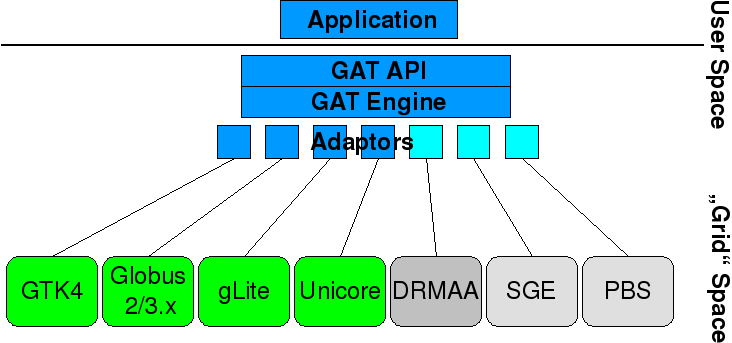
\includegraphics[width=.8\textwidth]{gat-arch}
  \caption{GAT Architecture}
  \label{abb:GATArchitecture}
\end{figure}


\section{How to get and install GAT\label{gatinst}}
\subsection{Download and installation of GAT}
GAT can be checked out from:

{\tt https://svn.aei.mpg.de/eScience/GridAPI/trunk/JavaGAT}

With the user \texttt{anonymous} and an empty password.

Before installing GAT, extract it to a directory of your choice.
The installation of GAT requires a Java SUN JDK version 6 or newer. There are two ways to install GAT:
\begin{enumerate}
\item installation of engine, adaptors, tests and javadoc in one step;
\item separate installation of the engine and the adaptors.
\end{enumerate}

\subsubsection{The one step installation}
For the one step installation:
\begin{enumerate}
\item Change to the directory, where you have extracted GAT to.
\item Set the environment variable {\tt GAT\_LOCATION} to point
  to this directory. If {\tt GAT\_LOCATION} is not set, the build
  process will fail!
\item Enter {\tt ant} to build the engine, the adaptors, some tests, and the
  documentation. 
\end{enumerate}

The documentation is of type javadoc, and the entry
page to this documentation is

{\tt \$GAT\_LOCATION/doc/javadoc/index.html}

The jar--files necessary for the GAT--Engine resides in {\tt
  \$GAT\_LOCATION/engine/lib}, those of the adaptors can be found in 
{\tt \$GAT\_LOCATION/engine/lib}

\subsubsection{Separate build}
If you are only interested in the engine and the adaptors, you can
build them separately. Before starting the build, please ensure that
the environment variable {\tt \$GAT\_LOCATION} points to the parent
directory of GAT. To build the engine change to the directory
{\tt \$GAT\_LOCATION/engine}, and enter {\tt ant}. For building the
adaptors, please change to {\tt \$GAT\_LOCATION/adaptors}, and again
enter ant. That's all.

\subsubsection{Build the supplemental AstroGrid packages}
The command line interfaces {\bf GATJobRun} and {\bf GATFileOps},
which have been developed within the AstroGrid--D project, must be
build separately. The build of the packages require a previous build of
the GAT engine and the GAT adaptors.

To build the {\bf GATJobRun} package, change to the directory
 
{\tt \$GAT\_LOCATION/astrogrid-packages/GATJobRun}, 

and enter 

{\tt ant -f build-standalone.xml}.

If you haven't installed a Sun Grid Engine (SGE) on your computer the
build process displays the message:

{\tt SGE\_ROOT = '/opt/SGE' found. If empty, you
can't submit jobs to SGE.\hfill\newline
Please set SGE\_ROOT and rebuild GATJobRun, if you like to use SGE}

This indicates that is is not possible to use the SGE adaptor of GAT
without an SGE on your computer.

For the {\tt GATFileOps} package please change to

{\tt \$GAT\_LOCATION/astrogrid-packages/GATFileOps}, 

and enter

{\tt ant -f build-standalone.xml}.

We recommend to have a look at the Readme files, before building the
packages.

\section{The Command Line Interface}
The command line interface (CLI) packages GATJobRun and GATFileOps
represent an extension to GAT. They have been developed within in
the AstroGrid project by the AEI in Potsdam--Golm.

\subsection{Submitting (Grid) jobs using the GATJobRun package}
The entry point to GATJobRun is the script {\tt gat-job-run} which is
located in the directory
 
{\tt \$GAT\_LOCATION/astrogrid-packages/GATJobRun/scripts}. 

It is
recommended to add this directory to the {\tt PATH} environment
variable, to enable an easy usage from everywhere directory in your 
system. If {\tt gat-job-run} is called without arguments, it prompts a
list of options and arguments:

{\tt
Missing host and/or executable string\hfill\newline
\hfill\newline
Usage: gat-job-run [OPTIONS] hostname executable [ARGUMENTS]\hfill\newline
\hfill\newline
OPTIONS:\hfill\newline
  -username      [STRING]     username for security context\hfill\newline
  -password      [STRING]     password for security context\hfill\newline
\hfill\newline
  -SubmitOnly    [true/false] submit only (true) or poll still exit\hfill\newline
\hfill\newline
  -stdin         [FILE]       path to input file\hfill\newline
  -stdout        [FILE]       path to output file\hfill\newline
  -stderr        [FILE]       path to error output file\hfill\newline
\hfill\newline
  -prestage      [FILE],...   path to prestage file(s) - comma separated\hfill\newline
  -poststage     [FILE],...   path to poststage file(s) - comma spearated\hfill\newline
\hfill\newline
  -RB.adaptor    [STRING]     force the use of a specific Resource Broker adaptor\hfill\newline
  -RB.jobmanager [STRING]     force the use of a specific Resource Broker jobmanager\hfill\newline
}

Some comments to the options / arguments.
\begin{itemize}
\item \begin{verbatim}hostname, executable\end{verbatim}: The name of the execution host, and
  the name of the executable. It is mandatory, to enter them.
\item {\tt -SubmitOnly}: The default behaviour of {\tt gat-job-run} is
  to submit a job, and to poll after the status of the job until it
  has finished. After the end of the job, {\tt gat-job-run}
  exits. This behaviour is only useful for short test jobs. In case
  of long term runs, it is desired that {\tt gat-job-run} exits before
  the job has finished. This can be achieved, by setting  {\tt
    SubmitOnly} to {\tt true}.
\item {\tt -RB.adaptor}: Here it is possible to enter the name of the
  GAT adaptor that shall be used for the job submission. If no
  adaptor is specified explicitly, GAT uses the first job
  submission adaptor which can be invoked successfully. The name of an
  adaptor is obtained by the name of its jar file without the
  suffix {\tt .jar} The GAT adaptors are located in 
  {\tt \$GAT\_LOCATION/adaptors/lib}. The name of the jar file which
  contains the gram adaptor is 
  {\tt GlobusResourceBrokerAdaptor.jar}. So if you like to invoke the
  gram adaptor of GAT you have to enter:

  {\tt -RB.adaptor GlobusResourceBrokerAdaptor}

\item {\tt -RB.jobmanager}: Enables to select the usage of a job manager
  as SGE or PBS. If no job manager is specified here, the default job
  manager will be invoked; usually this would be fork.
\end{itemize}

The script {\tt gat-job-run} consists mainly of the java call for the
GATJobRun package. However, you can define some variables for GAT in this
call; the most important one are:
\begin{itemize}
\item {\tt -Dgat.adaptor.path=<path name>} the name of the directory
  where the adaptors (there jar files) are located;
\item {\tt -Dgat.debug} set the logging level to debug, GAT writes
  debug and info messages to the console, very helpful in case of
  problems.
\end{itemize}  

\subsection{File operations with GATFileOps}
Like GATJobRun GATFileOps also uses a script as entry point. It is
called {\tt gat-file-operation}, and it is located in the directory
 
{\tt \$GAT\_LOCATION/astrogrid-packages/GATJobRun/scripts}. 

Again we
recommend to add this directory to the {\tt PATH}. Calling 
{\tt gat-file-operation} without arguments, will deliver list of
possible options and arguments:

{\tt
Usage: gat-file-operation [OPTIONS] <operation> <source> <dest>\hfill\newline
\hfill\newline
   OPTIONS:\hfill\newline
\hfill\newline
   -Adaptor   [STRING]   force the use of a specific file adaptor\hfill\newline
\hfill\newline
   <operation>: RemoteCopy, RemoteMove or DeleteFile\hfill\newline
   <source>:    source file\hfill\newline
   <dest>:      destination file; not used at <operation> DeleteFile\hfill\newline
}

The only option that is available is {\tt -Adaptor}, and it can be
used to force the usage of a special adaptor. The other arguments are
necessary for a call of {\tt gat-file-operation}, in order to obtain
the desired operation. 
\begin{itemize}
\item {\tt <operation>}: This argument can take the values 
{\tt RemoteCopy}, {\tt RemoteMove}, or {\tt DeleteFile}. 
{\tt RemoteCopy} copies a file, if desired from one grid host to
another; {\tt RemoteMove} moves a file through the grid, and 
{\tt DeleteFile} deletes a file anywhere in the grid.
\item {\tt <source>} The source file of the operation.
\item {\tt <dest>} The destination file of the operation. The
  destination file will be ignored in case of {\tt DeleteFile}.
\end{itemize}
Both {\tt <source>} and {\tt <dest>} can be file names or URIs,
dependent on where the files are located. In order to benefit of the
flexibility of GAT, Java--GAT offers its own protocol type ``{\tt
  any}''. So a {\tt RemotyCopy} call with {\tt gat-file-operation}
might look as follows:

{\tt gat-file-operation RemoteCopy
  any://localhost.de//home/ali/bin/test-geo600.sh \newline
\hspace*{5.86cm}  any://remotehost.de//tmp/tester.sh}

If {\tt any} is entered instead of {\tt file} or {\tt gsiftp}, any
adaptor that can be used for the copy will be invoked. Using {\tt gsiftp}
will force the usage of gridftp for the transfer.



\section{Programming against the GAT--API}
In this chapter we don't provide a description of the whole GAT--API,
this is left to the GAT documentation. However, because we
have developed job submission adaptors for gLite, Unicore, SGE, and PBS within the
AstroGrid project, we present two short examples describing the coding
against the GAT--API for file operations, and for job
submission.

\subsection{File operations on entire files with GAT}
If you like to copy a file from one URI (or file) to another, your
class might look as follows:

{\tt
1\hspace*{1cm} import org.gridlab.gat.*;\hfill\newline
2\hspace*{1cm}  import org.gridlab.gat.io.File;\hfill\newline
3\hfill\newline
4\hspace*{1cm}  public class RemoteCopy \{\hfill\newline
5\hspace*{2cm}      public static void main(String[] args) throws Exception \{\hfill\newline
6\hspace*{3cm}         GATContext context = new GATContext();\hfill\newline
7\hfill\newline
8\hspace*{3cm}          URI src = new URI(args[0]);\hfill\newline
9\hspace*{3cm}          URI dest = new URI(args[1]);\hfill\newline
10\hspace*{2,8cm}         File file = GAT.createFile(context, src);                // create file object\hfill\newline
11\hfill\newline
12\hspace*{2,8cm}         file.copy(dest);                                         // and copy it\hfill\newline
13\hspace*{2,8cm}         GAT.end();\hfill\newline
14\hspace*{1,8cm}      \}\hfill\newline
15\hspace*{0.8cm}\} \hfill\newline
}

Some comments to the code. To enable any further GAT operation, e.~g.~
the creation of GATFile or a GATResourceBroker (the latter is required
for the submission of jobs, you
need to create a new instance of the object {\tt GATContext}, as shown
in line 6.

The example class above is called with two arguments, namely the source, and
the destination file. These files must be given in an URI description,
e.g.~as {\tt ftp://10.0.0.1/output}. Of course you can use here also
the protocol type {\tt any://} for allowing GAT to use any protocol
(via available GAT adaptor) which
can be used for a file operation. This is the concept of {\bf late
  binding} realized in GAT. Due to this concept, GAT uses the first
adaptor for a file operation, which can invoked successfully. If it is
desired to force the usage of a specific adaptor, you must enter the
protocol you want to use, e.g.~ {\tt ftp://, gsiftp://, http://,
  file://,}, etc\dots

The GATFile inherits all methods of the
Java File class, and offers extensions as {\tt copy} or {\tt
  move}, and via the corresponing GAT adaptors it is possible to
perform file operations in a Grid environment. For a detailed description please look at the JavaDoc of
JavGAT. In our example the method {\tt copy} (line 12) is used, to copy the file. Every
GAT program should call {\tt GAT.end} before exiting the
class. This terminates all threads which might be still alive.

\subsection{Job submission with the ResourceBroker}
At the begin again a screenshot of an example class, which enables to
submit a job.

{\tt 
1\hspace*{1cm}import org.gridlab.gat.*;\hfill\newline
2\hspace*{1cm}import org.gridlab.gat.io.File;\hfill\newline
3\hspace*{1cm}import org.gridlab.gat.resources.*;\hfill\newline
4\hfill\newline
5\hfill\newline
6\hspace*{1cm}public class SubmitJob \{\hfill\newline
7\hspace*{2cm}    public static void main(String[] args) throws Exception \{\hfill\newline
8\hspace*{3cm}        GATContext context = new GATContext();\hfill\newline
9\hfill\newline
10\hfill\newline
11\hspace*{2,8cm}         URI LocalFile=new URI(args[0]);\hfill\newline
12\hspace*{2,8cm}         URI RemoteFile=new URI(args[0]);\hfill\newline
13\hspace*{2,8cm}         URI PostRemoteFile=new URI(args[0]);\hfill\newline
14\hspace*{2,8cm}        URI PostLocalFile=new URI(args[0]);\hfill\newline
15\hfill\newline
16\hspace*{2,8cm}         SoftwareDescription sd = new SoftwareDescription();\hfill\newline
17\hspace*{2,8cm}         sd.setExecutable("/bin/hostname");\hfill\newline
18\hspace*{2,8cm}         File stdout = GAT.createFile(context, "hostname.txt");\hfill\newline
19\hspace*{2,8cm}         sd.setStdout(stdout);\hfill\newline
20\hspace*{2,8cm}         sd.addPreStagedFile(GAT.createFilecontext,LocalFile),\hfill\newline
21\hspace*{7,1cm}       GAT.createFile(context,RemoteFile));\hfill\newline
22\hspace*{2,8cm}         sd.addPostStagedFile(GAT.createFilecontext,PostRemoteFile),\hfill\newline
23\hspace*{7,1cm}       GAT.createFile(context,PostLocalFile));\hfill\newline
24\hfill\newline
25\hspace*{2,8cm}         JobDescription jd = new JobDescription(sd);\hfill\newline
26\hfill\newline
27\hspace*{2,8cm}         String JobManagerContact = new String("any://" + "host.grid.org");\hfill\newline
28\hspace*{2,8cm}         ResourceBroker broker = GAT.createResourceBroker(context,\hfill\newline
29\hspace*{8,5cm}         new URI(JobManagerContact));\hfill\newline
30\hfill\newline
31\hspace*{2,8cm}         Job job = broker.submitJob(jd);\hfill\newline
32\hspace*{2,8cm}         while (job.getState() != Job.STOPPED \&\& \hfill\newline
33\hspace*{4,8cm}               job.getState() != Job.SUBMISSION\_ERROR) Thread.sleep(1000);\hfill\newline
34\hfill\newline
35\hspace*{2,8cm}         GAT.end();\hfill\newline
36\hspace*{2,8cm}    \}\hfill\newline
37\hspace*{1,8cm}\}\hfill\newline
38\hspace*{0,8cm}\}
}

To submit a job, you need to create a {\tt SoftwareDescription}, which
is required for the later creation of a 
{\tt JobDescription}, and the {\tt JobDescription} is the only argument
you need to create an instance of the {\tt ResourceBroker} class. 

Among others, the
{\tt SoftwareDescription sd} 

offers the following methods:
\begin{itemize}
\item {\tt sd.setExecutable("executable"}, to add the name of the executable;
\item {\tt sd.SetArguments(String[] jobargs)}, to add the executables arguments;
\item {\tt sd.setStdin(GATFile Input, sd.setStdout(GATFile
  Output)}), allows to define stdin and stdout,
\item {\tt sd.addPreStagedFile(GATFile File}, {\tt
  sd.addPostStagedFile(GATFile File}, can be used, to define files for
pre, and poststaging,
\item {\tt sd.addAttribute(String arg0, Object arg1)}, this method
  allows to add special attributes as the number od nodes or the
  memory required for the job. Please contact the adaptor developers
  if you are not sure, how this attributes must be called.
\end{itemize}

The  {\tt SoftwareDescription} contains a list of variables which must
be known, to execute the program
For a complete description please have a look at the Java documentation of
GAT.

The {\tt JobDescription} is necessary for submitting a job, checking
its status, killing it, etc\dots You can create this 
{\tt JobDescription} with the command:
        
{\tt JobDescription jd = new JobDescription(SoftWareDescription sd);}

The last step before submitting a job, is to get a 
{\tt ResourceBroker}. The {\tt ResourceBroker} requires the
information about the exeution host, given in an URI
representation. In the example above this information is given by {\tt
JobManagerContact} (line 27). Having defined the execution like this
the ResourceBroker is created by:

{\tt ResourceBroker broker = GAT.createResourceBroker(context, new URI(JobManagerContact);}

Having the the {\tt ResourceBroker broker} available, it is possible to
submit a job simply by:

{\tt Job job = broker.submitJob(jd);}

The {\tt Job} object  {\tt job} given back in case of a successful job
submission allows operations on the job, e.g.\ as:
\begin{itemize}
\item {\tt job.getState}, to check the status of the job;
\item {\tt job.stop}, to stop a job;
\item {\tt job.hold}, to hold a job;
\item {\tt job.resume}, to resume a job;
\item {\tt job.getExitStatus}, to get exit status of a job.
\end{itemize}

However, the final job scheduler must support these operations.


\section{Using Grid adaptors with GAT}
The usage of the Grid adaptors in GAT requires some configuration on
the computer, where these adaptors should be used. These
configurations only concerns providing the necessary certificates.

\subsection{The usage of the Globus adaptors of GAT}
To use the Globus adaptors it is necessary to provide the Globus Grid
certificates. There are two types of certificates which must be
available:
\begin{enumerate}
\item the personnel certificates {\tt userkey.pem}, and {\tt
    usercert.pem}, which must be located in the directory {\tt\$HOME/.globus};
\item the host certificates of the Grid hosts you like to access,
  which must be located in the directory
  {\tt\$HOME/.globus/certificates}.
\end{enumerate}

To create a proxy certificate you can use the {\tt grid-proxy-init}
(or {\tt grid-proxy-init.bat} on Windows) of
GAT, which is located in {\tt \$GAT\_LOCATION/bin}. The script invokes
the class {\tt org.globus.tools.ProxyInit} which is a
class of the Java Cog Kit, and delivered with GAT. This class reads in some configuration
information from the dataset {\tt \$HOME/.globus/cog.properties}, but
only if this file is available. {\tt cog.properties} might look as follows

\begin{verbatim}
#Java CoG Kit Configuration File
#Tue Aug 28 10:41:58 CEST 2007
usercert=/home/alibeck/.globus/usercert.pem
userkey=/home/alibeck/.globus/userkey.pem
proxy=/tmp/x509up_u1000
#cacert=/etc/grid-security/certificates
cacert=/home/alibeck/.globus/cog-certificates
\end{verbatim}

The single parameters have the following meaning:
\begin{itemize}
\item {\tt {\bf usercert}}: The path to the file containing your
  drid certificate.
\item {\tt {\bf userkey}}: The path to the file containing your
  Grid key.
\item {\tt {\bf proxy}}: The name under which your proxy
  certificate which you create with {\tt grid-proxy-init} is stored.
\item {\tt {\bf cacert}}: The path of the directory, which
  contains the host certificates.
\end{itemize}

Without any configurations in {\tt cog.properties}, the CoG
Toolkit will try to find the required files in default locations
according to the following rules:
\begin{itemize}
\item If the {\tt usercert} property is not set, first the
{\tt X509\_USER\_CERT} system property is checked. If the system
property is not set, the value defaults to
{\tt \$HOME/.globus/usercert.pem}.
\item If the {\tt userkey} property is not set, first the
{\tt X509\_USER\_KEY} system property is checked. If the system
property is not set, the value defaults to
{\tt \$HOME/.globus/userkey.pem}.
\item If the {\tt cacert} property is not set, first the
{\tt X509\_CERT\_DIR} system property is checked. If the system
property is not set, then the {\tt \$HOME/.globus/certificates}
 irectory is checked. If the directory does not exist, and
on a Unix/Linux machine, the directory with the name \linebreak[4] {\tt /etc/grid-security/certificates} is checked next.
If one of these directories with certificates is found, all
the certificates in that directory will be loaded and
used. If no directory is found, the Java CoG will not work.
\item If the {\tt proxy} property is not set, first the
{\tt X509\_USER\_PROXY} system property is checked. If the system
property is not set, then it defaults to a value based on
the following rules: If a {\tt UID} system property is set, and
running on a Unix/Linux machine it returns
{\tt /tmp/x509up\_u\$UID}. If any other machine then Unix/Linux,
it returns {\tt \$\{tempdir\}/x509up\_u\$\{UID\}}, where tempdir is a
platform--specific temporary directory as indicated by the
java.io.tmpdir system property. If a {\tt UID} system property is
not set, the username will be used instead of the {\tt UID}.
That is, it returns {\tt \$\{tempdir\}/x509up\_u\_\$\{username\}}.
\end{itemize}


\subsection{How to use the GAT-gLite Adaptor}

\subsubsection{Introduction}

Regarding security, the gLite adaptor behaves mostly like Globus. That
means, that a valid proxy impersonating the user on the Grid is
required. The difference with gLite, however, is that instead of an
entirely self-signed proxy, gLite uses so-called VOMS proxies for
authentication and authorization. VOMS proxies are enhanced Globus
proxies, that contain extensions signed  by a VOMS server about the
user's roles, group memberships and capabilities to simplify
authorization at the Grid site level and spare the site administrators
the task of updating huge user databases. In order to receive a VOMS
proxy, users must contact a VOMS server in a connection secured with a
Globus proxy and request certain roles, groups and capabilities. If
the user is a member in the VO (virtual organisation), that is
administered by the VOMS server, this request will either be granted
or denied based on the suitability of the user for the requested
memberships. If the request is granted, the server will generate a
signed certificate containing the granted request and store that in
the user's proxy. The user can now impersonate herself at Grid sites
belonging to the same VO as she does and will receive authorization
compliant to the granted capabilities.

\subsubsection{Configuration of the gLite adaptor}

To be able to make the VOMS-proxy request on behalf of the user, the gLite adaptor needs to know a few additional pieces of data:

\begin{itemize}
	\item The name of the VO for which the user wants to obtain a credential (e.g. nordugrid, knowarc, VOCE, ...)
	\item The endpoint of the VOMS server webservice (this address is usually different to the URL at which the VOMS admin can be accessed with a browser)
	\item The port at which the VOMS server is listening to requests
	\item The distinguished name (DN) of the VOMS Host. If you are
          unsure about this, you can usually find the information on
          the "Configuration" page in the VOMS admin server application. (Fig. \ref{vomsDN})
\end{itemize}

\begin{figure}\label{vomsDN}
	\begin{center}
	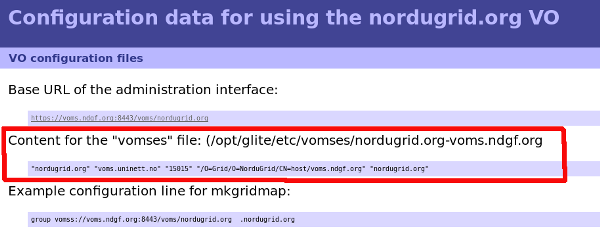
\includegraphics{vomsDN_small.png}
	\caption{The membership details page in the VOMS Admin gives you the DN of the VOMS host}
	\end{center}
\end{figure}

These values have to be specified as preferences of the current GAT context. Additionally, a CertificateSecurityContext with the path to the user certificate and key must be given. 

An example configuration of all the necessary parameters for the gLite adaptor could look as follows:

\begin{verbatim}
	GATContext context = new GATContext();
	CertificateSecurityContext secContext =
	    new CertificateSecurityContext(
	    new URI("/home/mustermann/.globus/userkey.pem"), 
	    new URI("/home/mustermann/.globus/usercert.pem"), 
	    "mysupersecretpwd");
		
	Preferences globalPrefs = new Preferences();
	globalPrefs.put("vomsServerURL", "skurut19.cesnet.cz");
	globalPrefs.put("vomsServerPort", "7001");
	globalPrefs.put("vomsHostDN", 
	                "/DC=cz/DC=cesnet-ca/O=CESNET/CN=skurut19.cesnet.cz");
	globalPrefs.put("VirtualOrganisation", "voce");
	context.addPreferences(globalPrefs);
	context.addSecurityContext(secContext);
\end{verbatim}

Please also note that a correct \verb+cog.properties+ file as in $<$insert reference to section about globus configuration here$>$ should be present.

\subsubsection{Optional configuration parameters}

\textbf{Security}

By default, the gLite-adaptor creates a VOMS proxy valid for 12
hours. If another validity period is desired, this behaviour can be
influenced by setting the \verb+vomsLifetime+ preference key. For example, if you want to set the lifetime to 1 hour, do:

\begin{verbatim}
	Preference globalPrefs = new Preferences();
	globalPrefs.put("vomsLifetime", "3600");
	context.addPreferences(globalPrefs);
\end{verbatim}

Please note, that the gLite adaptor will reuse any proxy that is valid
longer than \verb+vomsLifetime+ or 10 minutes, if \verb+vomsLifetime+
is not present.\footnote{The gLite adaptor will not perform automatic
  renewal, if the proxy times out during the execution of a job.} If
you want the adaptor to explicitly construct a new proxy every time a
job is submitted, you can instruct it to do so by setting the preference key glite.newProxy. For example

\begin{verbatim}
	Preference globalPrefs = new Preferences();
	globalPrefs.put("glite.newProxy", "true");
	context.addPreferences(globalPrefs);
\end{verbatim}

forces the gLite-adaptor to construct a new proxy for the submitted
job, even if an existing one is valid for a longer period than
\verb+vomsLifetime+. This behaviour is required, if you are submitting
to sites belonging to different VOs.

\textbf{Matchmaking}

Preferences influencing matchmaking decisions are set either as
SoftwareDescription attributes or as SoftwareResourceDescription and
HardwareResourceDescription properties, as previsioned in
JavaGAT. Most attributes are supported, but since the set of
previsioned attributes is somewhat tailored to Globus' RSL format,
this can only be done where the attributes can be translated to JDL in
a feasible way, or can be included as GLUE requirements. Table
\ref{attributes_JDL_table} gives an overview of the supported software
description attributes and how they are handled in the JDL document,
while table \ref{resource_JDL_table} shows how
SoftwareResourceDescription and HardwareResourceDescription properties
are translated to the JDL. If not noted otherwise, input parameters in
form of attributes or resource description properties are always strings and the comparison operator in the JDL is equality.

\begin{table}\label{attributes_JDL_table}
\begin{tabular}{|l|l|}
\hline
\textbf{SD attribute} & \textbf{Mapping to JDL} \\
\hline
time.max & other.GlueCEPolicyMaxWallClockTime \\
\hline
walltime.max & other.GlueCEPolicyMaxWallClockTime \\
\hline
cputime.max & other.GlueCEPolicyMaxCPUTime \\
\hline
project & HLRLocation \\
\hline
memory.min & other.GlueHostMainMemoryRAMSize $>=$ \\
\hline
memory.max & other.GlueHostMainMemoryRAMSize $<=$ \\
\hline
glite.retrycount & RetryCount \\
\hline
\multirow{4}{*}{glite.DataRequirements.InputData} & DataRequirements = \{ \\ 
 & [ DataCatalogType="RLS"; \\
 & InputData=\{...\} ] \} \\
 & DataAccessProtocol = \{https, gsiftp\};\} \\ 
\hline
\end{tabular}
\caption{List of SoftwareDescription attributes and their mapping to JDL}
\end{table}

\begin{table}\label{resource_JDL_table}
\begin{tabular}{|l|l|}
\hline
\textbf{ResourceRequirement} & \textbf{Mapping to JDL} \\
\hline
os.name & other.GlueHostOperatingSystemName \\
\hline
os.release & other.GlueHostOperatingSystemRelease \\
\hline
os.version & other.GlueHostOperatingSystemVersion \\
\hline
os.type & other.GlueHostProcessorModel \\
\hline
cpu.type & other.GlueHostProcessorModel \\
\hline
machine.type & other.GlueHostProcessorModel \\
\hline
machine.node = (String$|$List $<$String$>$) & other.GlueCEUniqueID \\
\hline
cpu.speed & other.GlueHostProcessorClockSpeed \\
\hline
memory.size & other.GlueHostMainMemoryRAMSize \\
\hline
disk.size & other.GlueSESizeFree \\
\hline
\multirow{2}{*}{glite.other} & any other.Glue* attributes here \\ & (that you specify yourself) \\
\hline 
\end{tabular}
\caption{List of SoftwareResourceRequirements and HardwareResourceRequirements and their mapping to JDL}
\end{table}

In gLite, matchmaking is supposed to be performed at the level of the workload management server (WMS), which acts as a meta-scheduling server. The WMS uses information stored in the information supermarket, which is usually also accessible from outside the WMS and can be used to perform manual preselections by the adaptor. For example, if you don't know the address of an WMS, but instead the address of your VOs LDAP information service, you can do:

\begin{verbatim}
	ResourceBroker rb = 
	       GAT.createResourceBroker(context, "ldap://is.example.com");
	Job job = rb.submitJob(jobDesc);
\end{verbatim}

The gLite adaptor will then try to retrieve a WMS accepting jobs for your VO from the LDAP server automatically and submit to this one, or, if more than one WMS accept jobs, submit to a random one of these. 

\textbf{Miscellenaeous configuration parameters}

By default, the gLite resource broker adaptor will delete the JDL file
created upon job submission. If you want to keep the JDL, e.g. for
debugging purposes, set the preference key glite.deleteJDL to false. 

The glite.pollIntervalSecs preference key determines how often the
gLite resource broker adaptor polls the logging \& bookkeeping service
for the current job's status. By default, this is 3 seconds.

For example, if you want to invoke the gLite adaptor with the setting
that the JDL files should be kept and that the L\&B server should be polled all 10 seconds, do the following:

\begin{verbatim}
	Preference globalPrefs = new Preferences();
	globalPrefs.put("glite.deleteJDL", "false");
	globalPrefs.put("glite.pollIntervalSecs", "10");
	context.addPreferences(globalPrefs);

\end{verbatim}

\subsection{How to use the GAT-Unicore Adaptor}

\subsubsection{Introduction}

The JavaGAT Unicore adaptor is based on  HilA\footnote{The HiLA
  package is described in
  http://www.unicore.eu/community/development/hila-reference.pdf.}
Therefore some HiLA specific configuration is necessary. This
configuration stuff is also described in this document.

\subsubsection{Installation}

The Unicore adaptor is now part of the regularly distributed adaptors, so
it is build during the default build process (see section \ref{gatinst}).

\subsubsection{Configuration of the HiLA}

The entry point for the configuration is the dataset {\tt unicore6.xml}. It might look as follows:
\scriptsize
\begin{verbatim}
<?xml version="1.0" encoding="UTF-8"?>

<!-- This is the default unicore6.xml. HiLAFactory will
� look for it on the classpath, if all else fails. -->
<!-- Use this file as an example unicore6.xml. -->

<beans xmlns:hila="http://www.unicore.eu/hila-unicore6">
� <hila:unicore6grid id="grid" outcomeDirectory="file:${user.home}/.hila/data" config="#config" />

� <hila-common:compositeconfig id="config" xmlns:hila-common="http://www.unicore.eu/hila-common">
� �<constructor-arg>
� � <list>
� �� <hila:registryconfig
       registryURL="https://zam461.zam.kfa-juelich.de:9117/AWARE-GROW/services/Registry?res=default_registry" grid="#grid" 
       securityProperties="#d-grid.security" />
� � </list>
� �</constructor-arg>
� </hila-common:compositeconfig>

� <bean name="d-grid.security" class="de.fzj.hila.implementation.unicore6.Unicore6SecurityProperties">
� � <constructor-arg value="/home/alibeck/.hila/d-grid.security" />
� </bean>

</beans>
\end{verbatim}
\normalsize

The path to this configuration file must be added as a definition while
calling the Java VM with the {\tt -D} flag, e.g.:

\begin{verbatim}
java -D/home/user/.hila/unicore.xml.
\end{verbatim}
 
Some notes to {\tt unicore.xml}:
\begin{itemize}
\item The outcomeDirectory defines the directory where all the results are stored. The default is \$HOME/.hila
\item The hila:registryconfig flag defines the security to be used (here d-grid.security), and the default 
registryURL:\hfill\newline
\footnotesize{\tt https://zam461.zam.kfa-juelich.de:9117/AWARE-GROW/services/Registry?res=default\_registry}\normalsize
\item Under the bean name {\tt d-grid.security} the
security issues are defined. The {\tt constructor-arg} value tag describes 
where security configuration can be found. This configuration file might look as follows:
\end{itemize}

\begin{verbatim}
unicore.wsrflite.ssl.keystore = /home/alibeck/certdir/alicert.jks
unicore.wsrflite.ssl.keypass = ****** 
unicore.wsrflite.ssl.keyalias = alip12cert
\end{verbatim}

{\tt keystore} \dots the name of the keystore file
{\tt keypass}  \dots the password of the keystore
{\tt keyalias} \dots the alias name of the key in the keystore which shall be used.

\subsubsection{How to get a keystore?}

We highly recommend to install portecle from

\begin{verbatim}http://portecle.sourceforge.net/\end{verbatim}

and use it with {\tt java -jar portecle.jar}. You are then in a graphical menu, which allows to

\begin{itemize}
\item create a new keystore
\item add your personal and your host certificates to it.
\end{itemize}

You need to add a p12-Key. However, this p12-key can be created from a pem-key using openssl.

{\bf IMPORTANT}: Right now, the keystore and the p12 certificate requires the same password. However, this will
be changed in the next HiLA release.

\end{document}